\graphicspath{ {figures/} }
\renewcommand{\myauthor}{Maximilian Koch}

Ein smartes Schachbrett vor sich zu haben ist an sich gut. Wenn sich jedoch auf diesem keine Software befindet, dann ist dessen Nutzung aber wenig vielversprechend. Ein Kernfeature ist das spielen gegen einen Schachcomputer

\subsection{Schachcomputer}
Um das was folgt besser zu verstehen, muss zuerst das Prinzip eines Schachcomputers erläutert werden. (?)



\subsection{Rotary encoder als Eingabegerät}
Zur Auswahl des passenden Eingabegeräts, kamen einige Vorschläge auf:
\begin{itemize}
	\item Das Steuern über vier Buttons, nach dem D-pad (Abkürzung für directional pad) Prinzip
	\item Über einen Joystick wie auf einem Konsolencontroller
	\item Über einen Rotary encoder, wie er zum Beispiel in Autos verbaut ist
\end{itemize}

Die schlussendliche Wahl fiel dann auf den Rotary encoder, da er eine gute Mischung aus modernität und funktionalität bietet. Bei dem Modell, welches im Schachbrett verbaut wurde, handelt es sich um den KY-040. Dieser ist der mit unter am weitesten verbreiteste seiner Art und die Einbindung mit dem Raspberry Pi 5 ist dank der gpiozero library auch praktisch.
\begin{figure}[h]
	\centering
	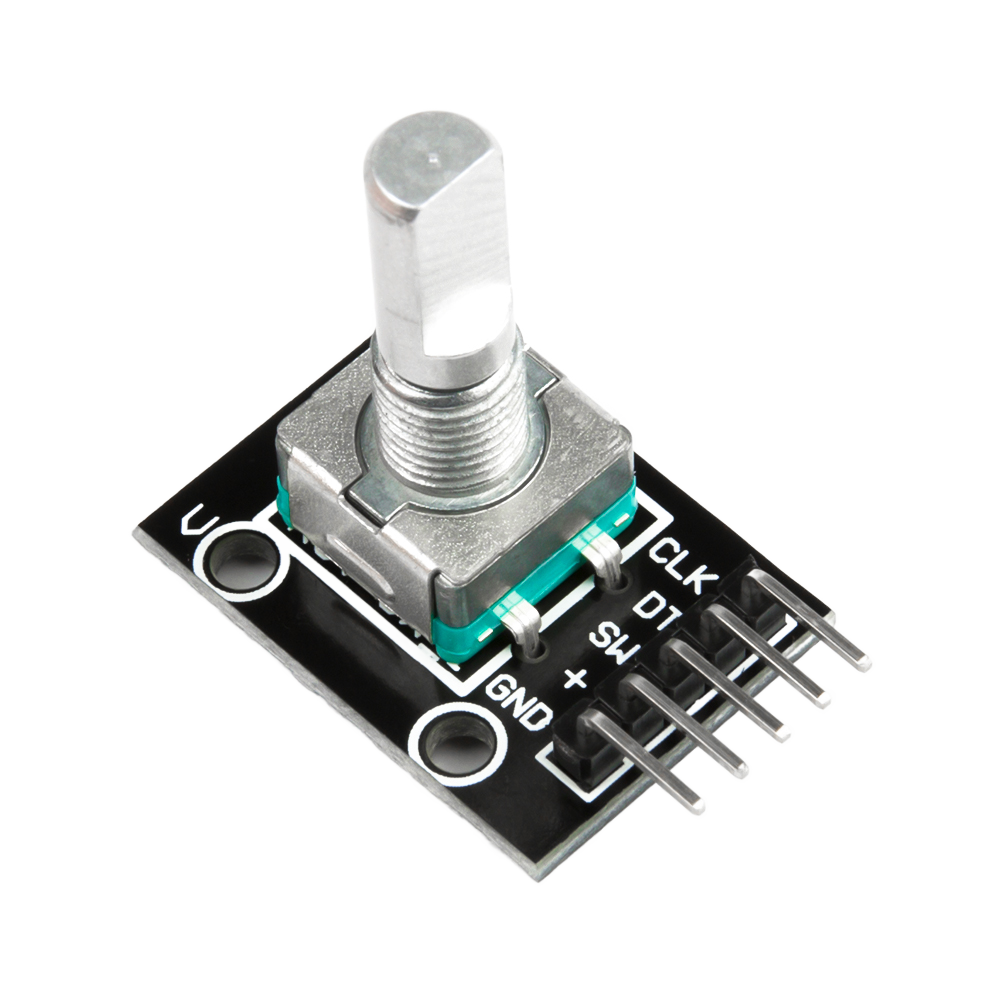
\includegraphics[width=6cm]{ky-040}
	\caption{KY-040 Rotary Encoder}
	\label{fig:ky040}
\end{figure}
%%https://www.elektronik-kompendium.de/sites/praxis/bauteil_ky040-drehschalter.htm

\subsubsection{Funktionsweise eines Rotary encoders}
Die Art, wie solch ein Inkrementalgeber funktionert, ist für viele auf den ersten Blick vielleicht nicht ganz verständlich und wird wahrscheinlich mit der Funktionweise eines Potentiometers verwechselt. Allerdings handelt es sich hier um einen kodierten Drehschalter. Der Hauptunterschied, welcher bei Bedienung schnell auffällt ist, dass sich dieses Bauteil, im Vergleich zum klassischen Potentiometer, \glqq unendlich lange\grqq{} drehen lässt. Jeder Drehpunkt kann taktil erfühlt werden.
Ein Inkrementalgeber hat zwei Ausgangssignale, A und B, welche bei Drehung ein periodisches Rechtecksignal ausgeben.

\begin{figure}[h]
	\centering
	\begin{minipage}[b]{0.6\textwidth}
		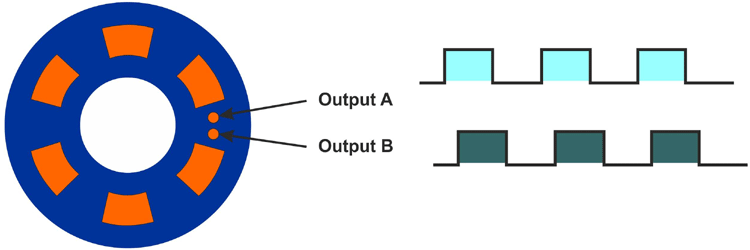
\includegraphics[width=\textwidth]{rotaryencoder_workings}
		\caption{Funktionsweise eines Inkrementalgebers}
		\label{fig:funkt}
		%%https://components101.com/modules/KY-04-rotary-encoder-pinout-features-datasheet-working-application-alternative
	\end{minipage}
	\hfill
	\begin{minipage}[b]{0.35\textwidth}
		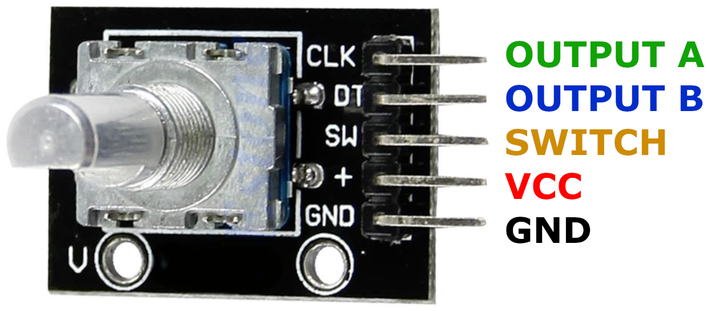
\includegraphics[width=\textwidth]{pinout}
		\caption{Pinout des KY-040}
		\label{fig:pinout}
		%%https://www.espboards.dev/sensors/ky-040/
	\end{minipage}
\end{figure}
Je nachdem, ob A oder B zuerst mit einer Zone Kontakt macht, wird eine Drehung in bzw. gegen die Uhrzeigerrichtung erkannt.



\subsubsection{Code für KY-040}

Der erste code sollte die Funktionalität sicherstellen und eine Vertrautheit mit dem Bauteil und dessen handling ermöglichen.
Auf der Dokumentationsseite von gpiozero findet sich unter Kapitel 2.21 \glqq Rotary encoder\grqq{} ein einfaches Beispiel mit einer LED. Mit Hilfe dieses Beispiels 

%\begin{adjustbox}{max width=\linewidth}
\begin{lstlisting}[style=Python, language=Python, captionpos=b, stepnumber=5, caption = {Erstes Beispiel für die Einbindung eines Rotary encoders}]
import threading

from gpiozero import RotaryEncoder, Button


class Encoder:
    def __init__(self):
        self.encoder = RotaryEncoder(13, 19, wrap = True,
									max_steps=100,
									bounce_time=0.05)

        self.button = Button(16, pull_up = True, 
							bounce_time = 0.05,
							hold_time = 2)

        self.done = threading.Event()

        self.button.when_released = self.handle_button  
        self.encoder.when_rotated = self.handle_rotate


    def handle_rotate(self):
        print(self.encoder.steps)


    def handle_button(self):
        print("Button released")

	
if __name__ == "__main__":
    encoder = Encoder()
    encoder.done.wait()
\end{lstlisting}
%\end{adjustbox}

\begin{figure}[h]
	\centering
	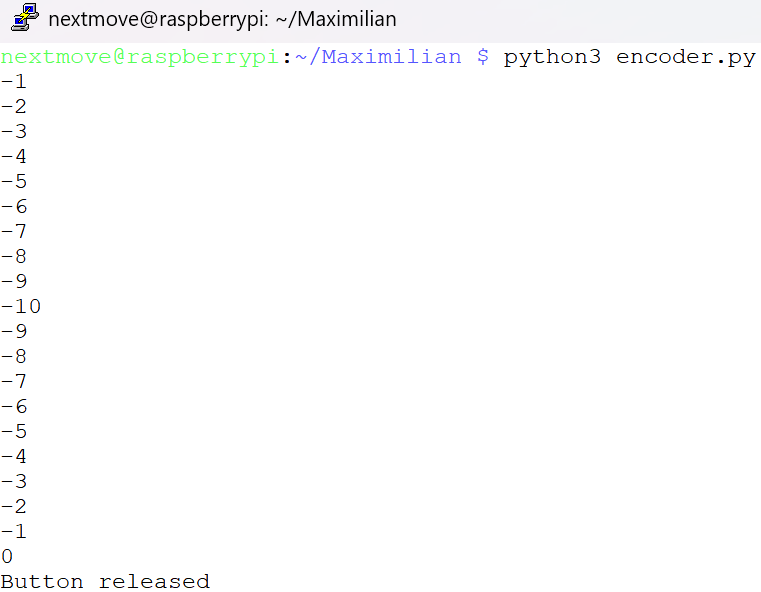
\includegraphics[width=\textwidth]{encoderCodeTest}
	\caption{Ergebnis des Code-Tests}
	\label{fig:encoderTest}
\end{figure}

Die Ausgabe zeigt, dass der Encoder korrekt funktioniert. Dreht man ihn im Uhrzeigersinn, so werden die Zahlen kleiner. Wird er in die entgegengesetzte Richtung gedreht, werden die Zahlen größer.
Am Ende wird nur der Button geklickt. Dieser Output wird mit \glqq Button released\grqq{} angezeigt. Es ist zu beachten, dass die Ausgabe der Schritte von 0 bis 100 geht, da im Code die Option \glqq max\char`_steps\grqq{} auf 100 gesetzt wurde. Ohne diese Option würde die Ausgabe von - inf bis +inf gehen, da sich der Encoder unendlich drehen lässt.

\subsection {Entwicklung eines Menüs}
Ein benutzerfreundliches Menü, welches zu Beginn des einschaltens erscheint, ist essenziell für ein gutes Spielerlebnis. Eine erste Überlegung, wie die Struktur dieses Spielmenüs aussehen soll, war wie folgt aufgebaut:
Wird das Schachbrett gestartet, wird auf einem Display, welches sich auf dem Schachbrett befindet, angezeigt, dass sich der Benutzer zwischen  \glqq Offlinespiel\grqq{} oder \glqq Onlinespiel\grqq{} entscheiden kann. 


\subsubsection{\glqq Offlinespiel\grqq{}}
Wird ersteres gewählt, so erscheint ein Untermenü. Hier besteht die Wahl zwischen \glqq Spieler vs. Spieler\grqq{} und \glqq Spieler vs. COM\grqq{} hat.
\glqq Spieler vs. Spieler\glqq{} steht dafür, dass der Benutzer gegen einen Gegenüber Schach spielen kann, ganz ohne Einmischung eines Schachcomputers. Im Falle der Entscheidung auf diese Möglichkeit, startet das Spiel sofort. Die Auswahl \glqq Spieler vs. COM\glqq{} hingegen erlaubt es, noch vor dem Beginn des Spiels zwischen eine von drei Schwierigkeitsstufen — Leicht, Mittel oder Schwer — zu wählen, welche der Schachcomputer haben soll. Die Stufen unterscheiden sich davon, wie lange der Schachcomputer Zeit lässt um einen optimalen Zug zu berechnen.
Nachdem eine Schwierigkeitsstufe gewählt wurde, geht nun das Spiel los und der Nutzer kann spielen.


\subsubsection{\glqq Onlinespiel\glqq{}}
Wird sich anstelle des Einzelspiels für das Onlinespiel entschieden, erscheint ein Untermenü, in dem der Benutzer aufgefordert wird, sich entwerder einzulogen oder einen neuen account zu registrieren. Ersteres geht davon aus, dass der Benutzer schon über ein Bentzerkonto verfügt und deshalb nur noch den NFC-Chip an das Lesegerät auf dem Schachbrett legen soll, damit der Benutzer in der Datenbank verglichen werden kann. Kann kein bereits bestehender Nutzer dem NFC-Chip zugeordnet werden, so wird der Nutzer infolgedessen aufgefordert, sich zu registrieren. Beim registrieren wird ein neuer Eintrag in der Datenbank erstellt, und der Benutzer kann fortfahren.
Im Falle des Onlinespiels kann der Spieler nur gegen einen Schachcomputer spielen und im Anschluss daran seine Partie auf der Website analysieren.


\subsubsection{Verknüpfen von Menü und Encoder}

\subsection{Die Restrukturierung}
UPDATE NACH RESTRUCTUNING
Wird das Schachbrett gestartet, wird auf einem Display, welches sich auf dem Schachbrett befindet, angezeigt, dass sich der Benutzer zwischen \glqq Login\glqq{} oder \glqq Registrieren\glqq{} entscheiden kann. Ersteres geht davon aus, dass der Benutzer schon über ein Bentzerkonto verfügt und deshalb nur noch den NFC-Chip an das Lesegerät auf dem Schachbrett legen soll, damit der Benutzer in der Datenbank verglichen werden kann. Kann kein bereits bestehender Nutzer dem NFC-Chip zugeordnet werden, wird der Benutzer aufgefordert, sich zu registrieren. Beim registrieren wird ein neuer Eintrag in der Datenbank gemacht, und der Benutzer kann fortfahren.


\subsection{Steuerung einer 2x2 Matrix}


\subsection{Spiellogik}

\subsubsection{Das Einzelspiel (Spieler gegen Computer)}

\subsubsection{Der Mehrspieler (Spieler gegen Spieler)}


\subsection{Einbindung des Spielererkennung}


\subsection{Die Datenübertragung}



